\section{The two assumptions that dominate}\label{sec:sensitivity}

\subsection{Realization}\label{sec:realization}

The Budget Lab's capital shock assumes AI leaves the realized share of
capital income unchanged, and they flag the assumption as a limitation.
It carries real weight: unrealized gains, retained earnings and accruals
inside retirement accounts never reach the individual tax base. Holding
Rapid~/~proportional fixed and varying only how much of the incremental
capital flow lands on a tax return (Figure~\ref{fig:realization},
Table~\ref{tab:realization} in the appendix), revenue runs from
\genRealZeroRev B at a 0\% realized share to \genRealFullRev B at their
100\% assumption --- linear to within a percent across a grid in
\genRealGridStepPct-point steps, with breakeven interpolated at a
\genRealBreakevenPct\% realized share (the grid's own adjacent points are
\genRealZeroRev B at 0\% and \genRealQuarterRev B at
\genRealGridStepPct\%). Below that, the household side of the fiscal system
loses money on Rapid AI growth: labor income still falls, and not enough
taxable capital income reaches returns to offset it.

One counterweight sits outside the household sector: corporate tax is levied
upstream of household realization, so the Budget Lab's corporate wedge would
still collect about \genTheirRapidCit B on the same shock regardless of the
realized share --- enough to keep the all-in total (household, state and
corporate) positive, about \genRealZeroAllIn B, even at the 0\% floor. Low
realization shifts the fiscal burden of an AI boom onto the corporate side;
it does not eliminate it. One scope note: the realization haircut applies
uniformly to all nine capital variables, including pass-through income and
retirement distributions that are realized by construction, so the low end
of the axis is a stress bound rather than a describable world.

Poverty is flat across the entire sweep, between \genRealPovMinPct\% and
\genRealPovMaxPct\%. Whether AI's capital gains are taxable moves the
federal balance sheet by more than a quarter-trillion dollars and moves poor
households essentially not at all: the transfer system responds to what
happens to wages, not to how much of the capital gain the tax system
reaches.

\begin{figure}[t]
\centering
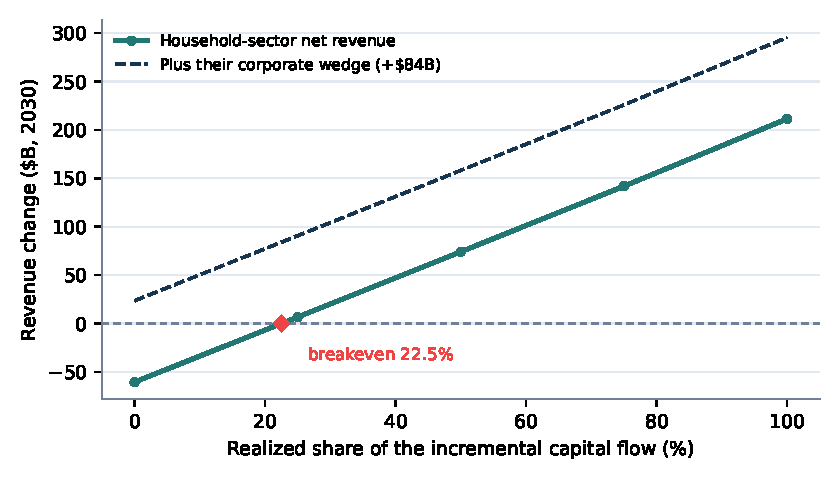
\includegraphics[width=0.8\textwidth]{figures/realization.pdf}
\caption{Net revenue under Rapid~/~proportional as the realized share of the
incremental capital flow varies. The dashed line adds the Budget Lab's
realization-independent corporate wedge.}
\label{fig:realization}
\end{figure}

\subsection{What counts as capital}\label{sec:scope}

Taxable pension and IRA distributions are taxed at ordinary rates. Counting
them in the capital set --- which the Budget Lab does, and the headline
results follow --- raises the revenue estimate and softens the ``capital is
taxed lightly'' mechanism. Excluding them (Table~\ref{tab:scope} in the
appendix) moves Rapid from \genRapidScopeFull B to \genRapidScopeExcl B and
flips Slow's sign (\genSlowScopeFull B to \genSlowScopeExcl B). Together
with realization, these two definitional choices span more of the revenue
answer than the choice between Slow, Moderate and Rapid.

\subsection{Stability across data builds}\label{sec:stability}

The results were first computed on the prior \texttt{populace-us} build
(build~o, 22 July 2026) and rerun on build~p (\genDataBuildDate{}, with
revised capital gains calibration) under the identical pinned model version
--- a data-only change. Both runs predate the Head Start correction noted
before the introduction, so this comparison uses the net-income accounting they
shared. No scenario revenue figure moved by more than
\$\genStabMaxAbsRevB B in absolute terms; in relative terms Moderate and
Rapid cells moved by at most \genStabMaxRelModRapidPct\%, while the smallest
Slow cells --- single-digit-billion bases --- moved by up to
\genStabMaxRelPct\%. Every poverty change moved by less than
\genStabMaxPovChangePp\,pp, and no conclusion changed. The recalibration's
visible effect is distributional: the baseline top-1\% net income share
rises from \genStabTopOneOld\% to \genStabTopOneNew\% (\genBaselineTopOnePct\%
after the correction), and New York's state
take under Rapid rises from \$\genStabNYOld B to \$\genStabNYNew B as more
of the gains land where they are taxed. This build-to-build movement bounds
sensitivity to data calibration, not sampling error, which is unquantified
here (Section~\ref{sec:discussion}). An average-tax-rate cross-check also
lands in range: Rapid~/~proportional turns a \genRapidPropMarketDelta B
market income increase into \genRapidPropRev B of receipts,
\genRapidPropATRPct\% --- of the same order as the 21--34\% band the Budget
Lab reports, though their denominator is gross factor income rather than
modelled market income.
